\indent \section{Моделирование модуля взаимодействия парсера русского языка с внешними базами знаний}

Моделирование --- исследование объектов познания на их моделях; построение и изучение моделей реально существующих объектов, процессов или явлений с целью получения объяснений этих явлений, а также для предсказания явлений, интересующих исследователя \cite{wiki_modelling}.

Модель --- система, исследование которой служит средством для получения информации о другой системе \cite{uemov}.

В этой главе представлен результат работы по моделированию модуля взаимодействия парсера русского языка и внешних БЗ (онтологий) в виде следующих видов моделей: концептуальные, информационные, структурные, функционально-структурные и алгоритмические. Локальной целью является получение пакета моделей, достаточного для начала проектирования модуля.

\subsection{Концептуальные модели}

Концептуальная (содержательная) модель --- это абстрактная модель, определяющая структуру моделируемой системы, свойства её элементов и причинно-следственные связи, присущие системе и существенные для достижения цели моделирования.

Для описания концептуальной модели используется фреймовый формализм, а именно описание концептуальной модели в соответствии с ролевым фреймом \cite{gold}.

Концепция = <Ф, П, С, Н, Ц>, где Ф --- основные функции системы, П --- путь реализации основных функций системы, С --- структурная основа системы, Н --- направленность функционирования, Ц --- цель функционирования.

\subsubsection{Общие концептуальные модели}

Для начала приведём общие концептуальные модели частей внешней среды, принимающих участие во взаимодействии посредством моделируемого модуля.

\textbf{Парсер} --- программный продукт, модуль или библиотека, функцией которого является синтаксический анализ входных последовательностей строк на естественном или формальном искусственном языке путём генерации дерева разбора, определения его принадлежности к языку и корректировки на основе формальной грамматики языка и алгоритма парсинга, направленный на дальнейшую автоматическую или автоматизированную обработку результата с целью извлечения знания.

\textbf{База знаний} --- информационная структура, база данных, функцией которой является хранение и оперирование знаниями (метаданными) о некоторой области знания посредством структурирования исходных фактов и логического вывода новых на основе правил продукции и принципов построения баз знаний, направленных на предоставление максимально полной информации с целью поддержки деятельности пользователя.

\textbf{Онтология} --- форма представления знаний, выполняющая функцию хранения детального описания некоторой области знания посредством структурирования классов объектов, связей между ними, их атрибутов и ограничений на основе спецификаций Semantic Web и языка OWL, направленных на формализацию предметной области с целью поддержки деятельности пользователя.

\subsubsection{Базово-уровневая концептуальная модель}

\textbf{Интерфейс онтология-парсер} --- программный модуль или библиотека, функциями которого являются организация доступа парсера к внешнему хранилищу знаний в виде онтологии, отправка запросов, трансляция в формат парсера и кэширование полученных ответов, передача парсеру необходимых правил продукции посредством получения исходного слова через прикладной программный интерфейс, генерации SPARQL-запроса по полученному слову, отправки запроса, разбору и временному хранению результата для передачи в алгоритм, на основе протоколов взаимодействия с семантичечкими хранилищами и спецификаций прикладного программного интерфейса парсера, направленный на увеличение релевантности, актуальности и корректности используемой парсером синтаксической информации с целью повышения качества обработки и снижения накладных расходов на модернизацию и/или новую разработку.

\subsection{Информационная модель модуля взаимодействия онтология-парсер}

Приведённая на рисунках \ref{fig:infomodel0} --- \ref{fig:infomodel3} информационная модель отображает иерархическое распределение информации по уровням её абстракции по мере декомпозиции структурных единиц моделируемого модуля.

\begin{figure}[H]
	\centering
		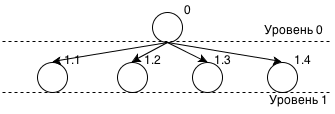
\includegraphics[scale=1.0]{images/infomodel0.png}
	\caption{\small Информационная модель, уровни 0 и 1}
	\label{fig:infomodel0}
\end{figure}

Обозначения на рисунке \ref{fig:infomodel0}: 0 --- рабочая информация модуля, 1.1 --- данные парсера, 1.2 --- информация в кэше, 1.3 --- внутренние данные генератора запросов, 1.4 --- данные онтологии.

\begin{figure}[H]
	\centering
		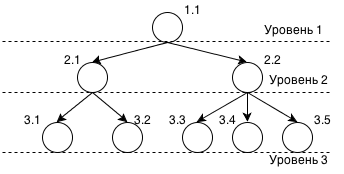
\includegraphics[scale=1.0]{images/infomodel1.png}
	\caption{\small Декомпозиция узла 1.1}
	\label{fig:infomodel1}
\end{figure}

Обозначения на рисунке \ref{fig:infomodel1}: 1.1 --- данные парсера, 2.1 --- исходные данные, 2.2 --- синтаксическая информация, 3.1 --- входная последовательность, 3.2 --- метаданные, 3.3 --- синтаксические структуры, 3.4 --- морфологические метки, 3.5 --- связи.

\begin{figure}[H]
	\centering
		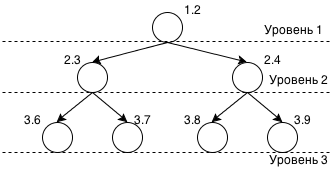
\includegraphics[scale=1.0]{images/infomodel2.png}
	\caption{\small Декомпозиция узла 1.2}
	\label{fig:infomodel2}
\end{figure}

Обозначения на рисунке \ref{fig:infomodel2}: 1.2 --- данные кэша, 2.3 --- ключи, 2.4 --- значения, 3.6 --- слова, 3.7 --- метки, 3.8 --- правила, 3.9 --- элементы запросов.

\begin{figure}[H]
	\centering
		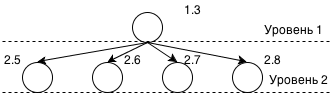
\includegraphics[scale=1.0]{images/infomodel3.png}
	\caption{\small Декомпозиция узла 1.3}
	\label{fig:infomodel3}
\end{figure}

Обозначения на рисунке \ref{fig:infomodel3}: 1.3 --- данные генератора/транслятора, 2.5 --- ключевые слова, 2.6 --- макеты запросов, 2.7 --- правила генерации запросов, 2.8 --- реквизиты доступа к внешней БЗ.

\subsection{Системно-структурная модель парсера русского языка}

Системно-структурные модели представляют моделируюмую систему в виде структурных блоков, связанных информационными либо материальными связями (путями прохождения информации).

На основе критики прототипа, приведённой в главе 1, и его структурной модели (рисунок \ref{fig:prototype_struct}), сформируем новую структурную модель, в которой учтём предложение по усовершенствованию прототипа. Модель представлена на рисунке \ref{fig:modifiedstruct}.

\begin{figure}[H]
	\centering
		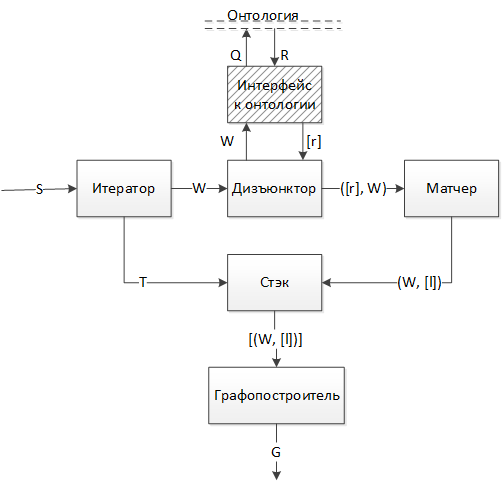
\includegraphics[scale=1.0]{images/modifiedstructure.png}
	\caption{\small Структурная модель модифицированного прототипа}
	\label{fig:modifiedstruct}
\end{figure}

На рисунке \ref{fig:modifiedstruct} добавляемый блок (Интерфейс к онтологии), замещающий собой блок прототипа Словарь, помечен штриховкой. Новые обозначения: Q --- SPARQL-запрос к онтологии, R --- ответ онтологии по запросу Q.

Декомпозиция блока Интерфейс к онтологии приведена на рисунке \ref{fig:decomposedstruct}.

\begin{figure}[H]
	\centering
		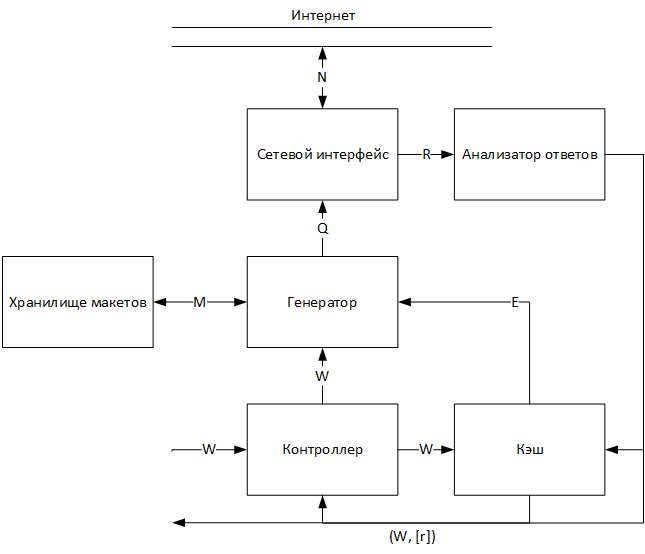
\includegraphics[scale=1.0]{images/decomposedstructure.png}
	\caption{\small Декомпозиция модуля Интерфейс к онтологии}
	\label{fig:decomposedstruct}
\end{figure}

Блок Контроллер принимает на вход слово W и выступает в роли ядра модуля, организующего связь между структурными элементами. Слово W передаётся в Кэш, откуда, если найдены, возвращаются правила для данного слова ([r]); в противном случае слово W передаётся Контроллером в Генератор запросов, использующий макеты (M) Хранилища макетов и кэшированные элементы E для генерации SPARQL-запроса Q, передаваемого в Сетевой интерфейс. Сетевой интерфейс взаимодействует с онтологией посредством двунаправленного потока сетевых пакетов (N), полученные данные (R) передаются в Анализатор ответов, преобразующий их в правила грамматики связей. Результат сохраняется в Кэш и передаётся в  Контроллер, возвращающий данные парсеру.


